% Drawing 154/06-5 -- folder 154, batch 06, archive page 107 (PDF page 108).
% Transcription: page presque vide : en haut à gauche, deux petits dessins en couleur, reprise des deux premiers de la page 106 : deux paires de droites orange, un faisceau de droites fléchées $\lambda$, $\alpha$, $\beta$, $\gamma$, l'arc $x_0 x_1$ noirci, et, à droite, la droite vert clair passant au-dessus du premier croisement, l'arc $x_0 x_1$ marqué au-dessous
% Kind: two pairs of crossings with arrowed lines; the line passing over the first crossing. Method 2 (schematic redraw from the facsimile). Status: ok.
% Notes: Top left, two small drawings repeating the first two of p. 106: two pairs of orange lines crossing, a pencil of arrowed lines lambda, alpha, beta, gamma (the labels read « lambda - beta mu » at this size; given as on p. 106), the arc x_0 x_1 blackened; and to the right the light green line passing over the first crossing, the arc x_0 x_1 marked below. Pencil hatching left out. Read from the page view.
% Coordinates: 1 unit = 1 mm = 1/100 of the crop width (bbox in page fractions: [0.157, 0.089, 0.547, 0.175]).
% Redrawn by Claude (claude-opus-5-5), issue #73, 2026-11-07; not checked by a human; not compiled (no TeX in the session).
% Revised by Claude (claude-opus-5-5) 2026-11-09 (issue #128) after Michel's check: vertices snapped to exact intersections (drawn points on their lines, meeting ends on the stroke they meet, near-concurrent lines through one computed point, curve ends on their rim); labels at \small as in folder 80 batch 3. Status: ok.
% Rights: reproduces part of the work -- behind RENDER_TRANSCRIPTS, never published by itself.
\documentclass[tikz,border=3pt]{standalone}
\usepackage{amsmath,amssymb}
\usetikzlibrary{patterns,arrows.meta}
\tikzset{Or/.style={orange!90!black}, Ye/.style={yellow!80!orange}, Lg/.style={green!60!black!70}, Dg/.style={green!45!black}, Br/.style={brown!80!black}, Rd/.style={red!85!black}, Bl/.style={blue!70!black}, Gy/.style={black!40}, pencil/.style={black!45}, struck/.style={black!35}, mark/.style={circle,draw,inner sep=1.3pt}, pt/.style={circle,fill,inner sep=0.9pt}, opt/.style={circle,draw,fill=white,inner sep=1.1pt}}
\colorlet{Or}{orange!90!black}\colorlet{Ye}{yellow!80!orange}\colorlet{Lg}{green!60!black!70}\colorlet{Dg}{green!45!black}\colorlet{Br}{brown!80!black}\colorlet{Rd}{red!85!black}\colorlet{Bl}{blue!70!black}\colorlet{Gy}{black!40}
\begin{document}
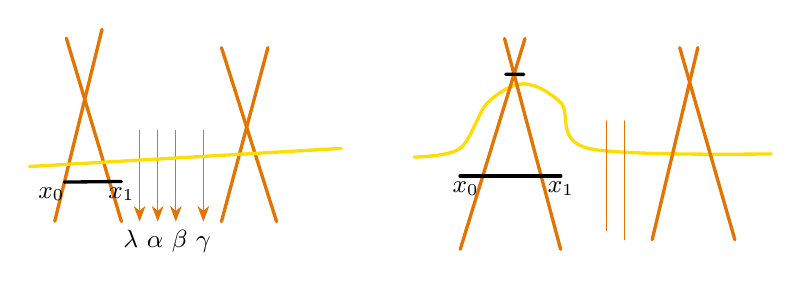
\begin{tikzpicture}[x=1mm,y=1mm,line cap=round,line join=round,font=\scriptsize]
\draw[Or,very thick] (5.53,-25.54) -- (11.53,-1.18);
\draw[Or,very thick] (7,-2.3) -- (14,-25.6);
\draw[Or,very thick] (26.7,-3.5) -- (33.7,-25.6);
\draw[Or,very thick] (32.6,-3.5) -- (26.7,-25.6);
\draw[Or,-{Stealth[length=2mm]}] (16.3,-14) -- (16.3,-25.6);
\draw[Or,-{Stealth[length=2mm]}] (18.6,-14) -- (18.6,-25.6);
\draw[Or,-{Stealth[length=2mm]}] (20.9,-14) -- (20.9,-25.6);
\draw[Or,-{Stealth[length=2mm]}] (24.4,-14) -- (24.4,-25.6);
\draw[Ye,very thick] (2.3,-18.6) -- (41.9,-16.3);
\draw[very thick] (6.75,-20.58) -- (14,-20.5);
\node[inner sep=1pt] at (5.1,-22.1) {\small $x_0$};
\node[inner sep=1pt] at (14,-22.1) {\small $x_1$};
\node[inner sep=1pt] at (19.8,-28.1) {\small $\lambda\ \alpha\ \beta\ \gamma$};
\draw[Ye,very thick] plot[smooth, tension=0.55] coordinates {(51.2,-17.4) (57,-16.3) (60.5,-10.5) (65.1,-8.1) (69.8,-10.5) (73.3,-16.3) (96.5,-17)};
\draw[Or,very thick] (57.03,-29.11) -- (65.25,-2.35);
\draw[Or,very thick] (62.65,-2.34) -- (69.77,-29.11);
\draw[very thick] (62.8,-6.89) -- (65.1,-6.9);
\draw[Or] (75.6,-12.8) -- (75.6,-26.7);
\draw[Or] (77.9,-12.8) -- (77.9,-27.9);
\draw[Or,very thick] (81.4,-27.9) -- (87.2,-3.5);
\draw[Or,very thick] (84.9,-3.5) -- (91.9,-27.9);
\draw[very thick] (57,-19.8) -- (69.8,-19.8);
\node[inner sep=1pt] at (57.7,-21.4) {\small $x_0$};
\node[inner sep=1pt] at (69.8,-21.4) {\small $x_1$};
\end{tikzpicture}
\end{document}
